\section{Method}\label{sec:method}
Given an input sequence $x = (x_1, \dots, x_n)$ with $x_i \in \mathbb{R}^{d}$, we compute queries $Q = XW^Q$, keys $K = XW^K$ and values $V = XW^V$, where $W^Q \in \mathbb{R}^{d \times d_k}$. The scaled dot-product attention is
\begin{equation}\label{eq:attn}
\mathrm{Attention}(Q,K,V) = \mathrm{softmax}\!\left(\frac{QK^\top}{\sqrt{d_k}}\right)V .
\end{equation}
As shown in Eq.~\eqref{eq:attn}, the factor $1/\sqrt{d_k}$ prevents the softmax from saturating when $d_k$ is large, e.g.\ $d_k = 64$. Following \cite{vaswani2017,he2016}, we add residual connections so that $y = x + f(x)$, and the loss is
\begin{equation}\label{eq:loss}
\mathcal{L}(\theta) = -\frac{1}{N}\sum_{i=1}^{N} \log p_\theta(y_i \mid x_i) + \lambda \lVert \theta \rVert_2^2 ,
\end{equation}
with $\lambda = 0.01$. The learning rate follows $\eta_t = d^{-0.5} \cdot \min(t^{-0.5}, t \cdot w^{-1.5})$ for warmup $w = 4000$ steps.\footnote{We found warmup essential; without it training diverged in 3 of 5 runs.}

\section{Experiments}\label{sec:exp}
We train on WMT 2014 English--German, which contains about 4.5 million sentence pairs, and report BLEU in Table~\ref{tab:res}. Our model reaches 28.4 BLEU, outperforming the best previous result by 2.0 points while costing only $3.3 \times 10^{18}$ FLOPs. Figure~\ref{fig:curve} shows that the validation loss decreases monotonically. The improvement is statistically significant ($p < 0.05$), although it may not generalize to low-resource pairs, as discussed in Section~\ref{sec:method}.

\begin{table}[t]\centering
\caption{BLEU scores and training cost on newstest2014.}\label{tab:res}
\begin{tabular}{llcc}\toprule
\multirow{2}{*}{Model} & \multirow{2}{*}{Size} & \multicolumn{2}{c}{BLEU} \\ \cmidrule(lr){3-4}
 & & EN-DE & EN-FR \\ \midrule
ByteNet & 1.2B & 23.75 & -- \\
ConvS2S & 0.9B & 25.16 & 40.46 \\
Ours (base) & 65M & 27.3 & 38.1 \\
Ours (big) & 213M & \textbf{28.4} & \textbf{41.8} \\ \bottomrule
\end{tabular}\end{table}

\begin{figure}[t]\centering
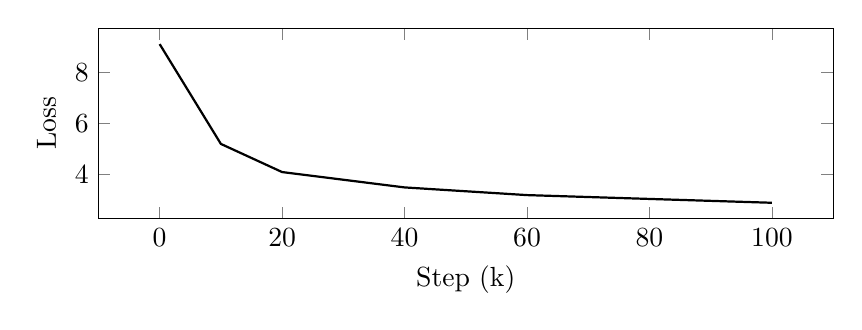
\begin{tikzpicture}\begin{axis}[width=0.9\columnwidth,height=4cm,xlabel={Step (k)},ylabel={Loss}]
\addplot[thick] coordinates {(0,9.1) (10,5.2) (20,4.1) (40,3.5) (60,3.2) (100,2.9)};
\end{axis}\end{tikzpicture}
\caption{Validation loss during training of the big model.}\label{fig:curve}
\end{figure}

Long paragraph to cross columns. The encoder is composed of a stack of $N = 6$ identical layers. Each layer has two sub-layers: the first is a multi-head self-attention mechanism, and the second is a simple, position-wise fully connected feed-forward network with inner dimension $d_{ff} = 2048$. We employ a residual connection around each of the two sub-layers, followed by layer normalization \cite{ba2016}. That is, the output of each sub-layer is $\mathrm{LayerNorm}(x + \mathrm{Sublayer}(x))$. To facilitate these residual connections, all sub-layers in the model, as well as the embedding layers, produce outputs of dimension $d_{model} = 512$. The decoder is also composed of a stack of $N = 6$ identical layers, and we modify the self-attention sub-layer to prevent positions from attending to subsequent positions; this masking ensures that predictions for position $i$ can depend only on the known outputs at positions less than $i$.
